\subsection{First Experience}

\subsubsection{Capturing packets from an execution of traceroute}
wasa

\subsubsection{Basic IPv4}
wasa

\subsubsection{Fragmentation}

This section of the experience was done on a Windows machine, and so we had to
work with the downloaded trace file.

First, we looked for the first IP datagram containing the first part of the
segment sent to the server. After finding it (it wasn't the first packet), we
looked for any field that might indicate that it was fragmented.

\begin{figure}[htbp]
    \centering
    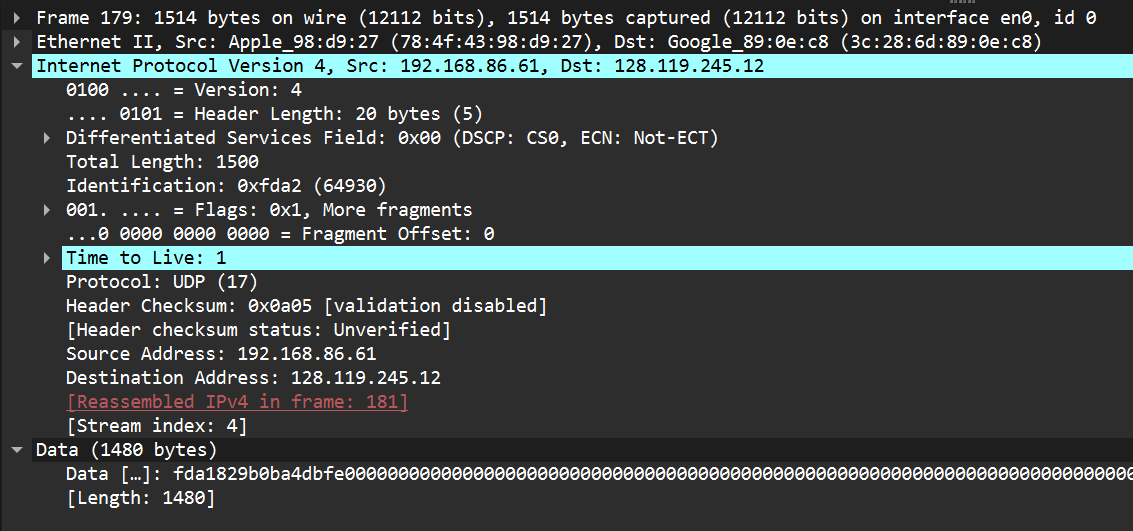
\includegraphics[width=1\linewidth]{img/1/3_1.png}
    \caption{First fragment}\label{fig:exp1_3_1}
\end{figure}

We can see that the flag \textbf{More Fragments} is set, and thus we can
conclude that the packet is indeed fragmented.

We then wanted to know if this packet was the first fragment, or a latter one.
Seeing that the \textbf{fragment offset} value is zero, we can conclude that
this is the first fragment.

The total number of bytes in this datagram (payload plus header) is 1480 plus
20, i.e. 1500, as shown in the previous image.

Moving on to the second fragment, we can see that the fragment offset is no
longer zero. This implies that this fragment is not the first one (which is
true).

\begin{figure}[htbp]
    \centering
    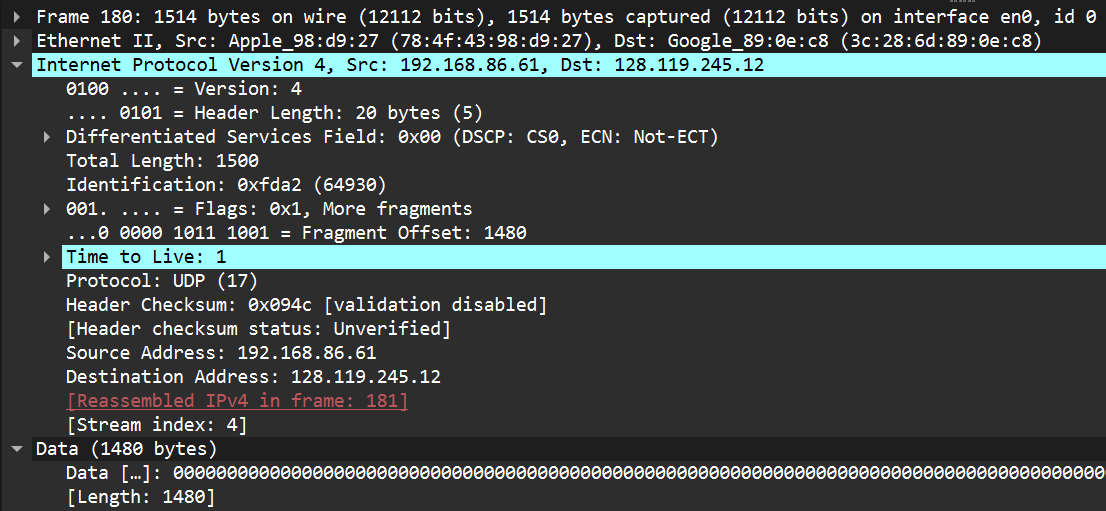
\includegraphics[width=1\linewidth]{img/1/3_2.png}
    \caption{Second fragment}\label{fig:exp1_3_2}
\end{figure}

If we compare the first and second fragments, we can identify the following
differences:

\begin{itemize}
    \item Fragment offset: 0 for first, 1480 for second
    \item Header checksum: different values as the fragment offset is different
\end{itemize}

Finally, we observed the third's fragment information. We immediately notice
that the flag values are different. In this case, the flag \textbf{more
    fragments} is unset, which implies that this is indeed the last fragment.

\begin{figure}[htbp]
    \centering
    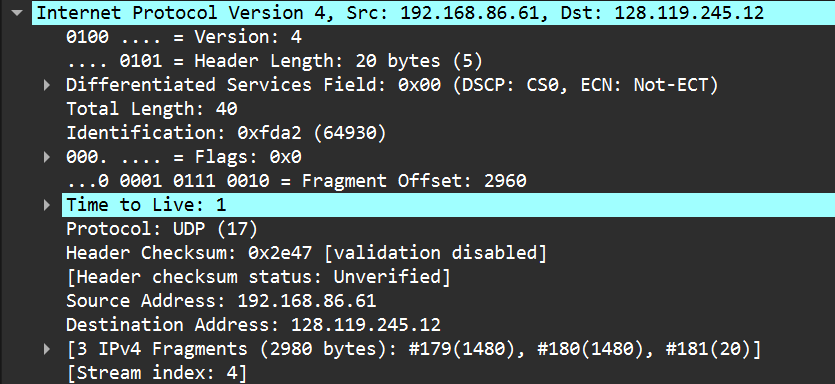
\includegraphics[width=1\linewidth]{img/1/3_3.png}
    \caption{Third fragment}\label{fig:exp1_3_3}
\end{figure}